\documentclass{beamer}
\usetheme{Madrid}
\usecolortheme{default}
\usepackage[utf8]{inputenc}
\usepackage{amsmath}
\usepackage{amsfonts}
\usepackage{amssymb}
\usepackage{tikz}
\usepackage{xcolor}
\usepackage{hyperref}

\title{CRISC Exam - Hard Concepts \& Exam Traps}
\subtitle{Section 3: Risk Response and Reporting Deep Dive Tutorial}
\author{CRISC Mastery Series}
\date{\today}

\begin{document}
	
	% ============================================================
	% TITLE SLIDE
	% ============================================================
	\begin{frame}
		\titlepage
	\end{frame}
	
	% ============================================================
	% OUTLINE
	% ============================================================
	\begin{frame}{Section 3 Tutorial Outline}
		\tableofcontents
	\end{frame}
	
	% ============================================================
	% SECTION 1: RISK RESPONSE STRATEGIES
	% ============================================================
	\section{1. Risk Response Strategies}
	
	% ----------------------------------------------------------------------
	\subsection{1.1 The Four Response Strategies}
	\begin{frame}{1.1 The Four Risk Response Strategies}
		\begin{block}{The Response Matrix}
			\begin{center}
				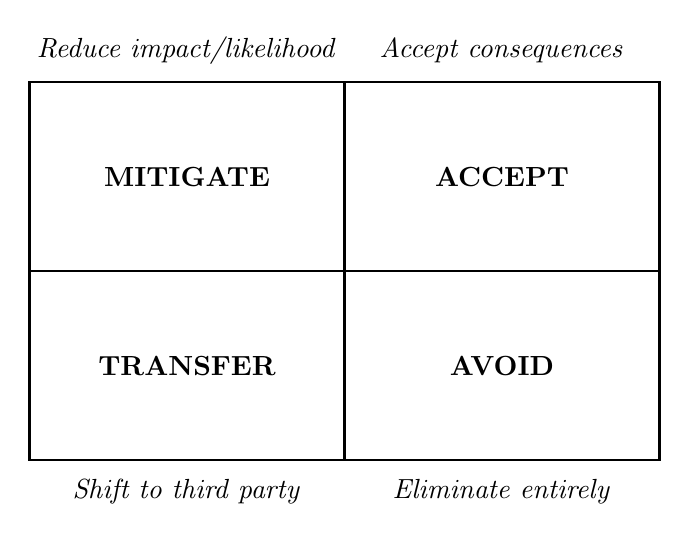
\begin{tikzpicture}[scale=0.8]
					% Four quadrants
					\draw[thick] (0,0) rectangle (5,3) node[pos=.5] {\textbf{MITIGATE}};
					\draw[thick] (5,0) rectangle (10,3) node[pos=.5] {\textbf{ACCEPT}};
					\draw[thick] (0,-3) rectangle (5,0) node[pos=.5] {\textbf{TRANSFER}};
					\draw[thick] (5,-3) rectangle (10,0) node[pos=.5] {\textbf{AVOID}};
					
					% Labels
					\node at (2.5,3.5) {\textit{Reduce impact/likelihood}};
					\node at (7.5,3.5) {\textit{Accept consequences}};
					\node at (2.5,-3.5) {\textit{Shift to third party}};
					\node at (7.5,-3.5) {\textit{Eliminate entirely}};
				\end{tikzpicture}
			\end{center}
		\end{block}
		
		\begin{alertblock}{The Critical Trap}
			\textbf{AVOID} is the \textbf{ONLY} strategy that eliminates risk entirely!
			All other strategies leave some \textbf{residual risk}.
		\end{alertblock}
	\end{frame}
	
	\begin{frame}{1.1 Mitigate}
		\begin{block}{Risk Mitigation}
			\begin{itemize}
				\item Manage risk through \textbf{countermeasures} and \textbf{controls}
				\item Cost of mitigation must be \textbf{less than} the effective risk
				\item Objective: Bring risk to \textbf{acceptable level}, NOT eliminate
			\end{itemize}
		\end{block}
		
		\begin{block}{Examples}
			\begin{itemize}
				\item Installing \textbf{anti-malware} software
				\item Performing \textbf{regular backups}
				\item \textbf{Patching} systems periodically
				\item Documenting and testing \textbf{incident response} plans
				\item Implementing \textbf{firewalls} and \textbf{IDS}
			\end{itemize}
		\end{block}
		
		\begin{alertblock}{The Critical Trap}
			\textbf{Mitigation} does NOT mean eliminating the risk. \\
			\textbf{Objective}: Reduce residual risk to within \textbf{acceptable tolerance}.
		\end{alertblock}
	\end{frame}
	
	\begin{frame}{1.1 Accept}
		\begin{block}{Risk Acceptance}
			\begin{itemize}
				\item Decision to accept risk based on \textbf{risk appetite} and \textbf{tolerance}
				\item \textbf{Formal decision} by senior management
				\item Must be \textbf{documented} and \textbf{reviewed} annually
				\item Risk can be within or outside appetite but \textbf{must NOT exceed capacity}
			\end{itemize}
		\end{block}
		
		\begin{block}{Examples}
			\begin{itemize}
				\item Not patching a \textbf{non-critical} system
				\item Continuing to use \textbf{end-of-life} software that is easily replaceable
				\item Accepting minor risks that cost more to fix than the potential loss
			\end{itemize}
		\end{block}
		
		\begin{alertblock}{The Critical Trap}
			\textbf{Acceptance} does NOT mean \textbf{ignoring} risk!
			\begin{itemize}
				\item Must be \textbf{formally documented}
				\item Must be approved by \textbf{senior management}
				\item Must be \textbf{reviewed periodically}
				\item Must have \textbf{compensating controls} if needed
			\end{itemize}
		\end{alertblock}
	\end{frame}
	
	\begin{frame}{1.1 Transfer}
		\begin{block}{Risk Transfer}
			\begin{itemize}
				\item Assign risk to another enterprise or partner
				\item Usually through \textbf{insurance} or \textbf{outsourcing}
				\item Better for risks with \textbf{low likelihood} and \textbf{high impact}
				\item Outcome: \textbf{Monetary indemnity} but reputational loss remains
			\end{itemize}
		\end{block}
		
		\begin{block}{Examples}
			\begin{itemize}
				\item \textbf{Cyber insurance} from an insurance provider
				\item Sharing security responsibility with \textbf{SaaS providers}
				\item Outsourcing to a \textbf{third-party vendor}
			\end{itemize}
		\end{block}
		
		\begin{alertblock}{The Critical Trap}
			\textbf{Transfer} does NOT eliminate risk! \\
			The organization is \textbf{still accountable} for the risk. \\
			\textbf{Reputational damage} remains even with insurance.
		\end{alertblock}
	\end{frame}
	
	\begin{frame}{1.1 Avoid}
		\begin{block}{Risk Avoidance}
			\begin{itemize}
				\item \textbf{Eliminate} the risk entirely
				\item \textbf{Terminate} the activities that give rise to risk
				\item \textbf{Irreversible} decision - extreme caution required
				\item Requires \textbf{senior management} approval
			\end{itemize}
		\end{block}
		
		\begin{block}{Examples}
			\begin{itemize}
				\item \textbf{Terminating} a project due to resource constraints
				\item \textbf{Shutting down} an office location due to natural hazards
				\item \textbf{Not engaging} in e-commerce altogether
			\end{itemize}
		\end{block}
		
		\begin{alertblock}{The Critical Trap}
			\begin{itemize}
				\item \textbf{Avoidance} is the \textbf{ONLY} strategy that eliminates risk
				\item Should only be used when risk \textbf{cannot be addressed} by other strategies
				\item Often \textbf{irreversible} - consider carefully!
			\end{itemize}
		\end{alertblock}
	\end{frame}
	
	% ----------------------------------------------------------------------
	\subsection{1.2 Response Selection Criteria}
	\begin{frame}{1.2 How to Select a Response}
		\begin{block}{Selection Factors}
			\begin{itemize}
				\item Risk \textbf{category} (Critical/High/Medium/Low)
				\item \textbf{Cost} of associated risks
				\item \textbf{Cost} of risk response
				\item \textbf{Availability} of controls
				\item Available \textbf{skillsets}
				\item \textbf{Complexity} of implementing controls
				\item \textbf{Resources} and \textbf{budgeting}
				\item \textbf{Alignment} with organizational strategy
				\item \textbf{Compatibility} with current controls
				\item \textbf{Contractual} requirements
				\item \textbf{Legal} and \textbf{regulatory} requirements
			\end{itemize}
		\end{block}
	\end{frame}
	
	\begin{frame}{1.2 Cost-Benefit Decision Logic}
		\begin{block}{The Decision Framework}
			\begin{itemize}
				\item \textbf{If Cost of Control < Expected Loss}: Implement control (Mitigate)
				\item \textbf{If Cost of Control > Expected Loss}: Accept risk or Transfer
				\item \textbf{If Risk Exceeds Risk Appetite}: MUST Mitigate or Transfer
				\item \textbf{If Risk Exceeds Risk Capacity}: MUST Avoid
			\end{itemize}
		\end{block}
		
		\begin{exampleblock}{Classic Exam Scenario}
			\textbf{Scenario}: Anti-malware cost exceeds loss expectancy of malware threats.
			
			\textbf{Most viable response}: \textbf{Risk Acceptance}
			
			\textbf{Why}: When cost of mitigation exceeds expected loss, the business case doesn't justify spending.
		\end{exampleblock}
	\end{frame}
	
	% ============================================================
	% SECTION 2: RISK OWNERS AND CONTROL OWNERS
	% ============================================================
	\section{2. Risk Owners and Control Owners}
	
	% ----------------------------------------------------------------------
	\subsection{2.1 Understanding Ownership}
	\begin{frame}{2.1 Risk Owners}
		\begin{block}{What is a Risk Owner?}
			\begin{itemize}
				\item Accountable individual for \textbf{risk treatment}
				\item Provides \textbf{budget} and \textbf{resources}
				\item Has \textbf{authority} to approve risk response
				\item \textbf{Owns the loss} if risk materializes
				\item Should be a \textbf{manager} or \textbf{executive}
			\end{itemize}
		\end{block}
		
		\begin{alertblock}{The Critical Trap}
			\textbf{Common Mistake}: Thinking IT owns risk.
			
			\textbf{Correct}: The \textbf{BUSINESS OWNER} owns the risk.
			
			\textbf{Why}: Risk impacts business objectives; IT is an enabler.
		\end{alertblock}
		
		\begin{block}{Without a Risk Owner}
			\begin{itemize}
				\item Hard to find accountable individual
				\item Risks may go \textbf{unnoticed}
				\item No one to approve \textbf{risk response}
				\item \textbf{Accountability} is diluted
			\end{itemize}
		\end{block}
	\end{frame}
	
	\begin{frame}{2.1 Control Owners}
		\begin{block}{What is a Control Owner?}
			\begin{itemize}
				\item Person who \textbf{implements} the control
				\item Responsible for \textbf{oversight} of control effectiveness
				\item Ensures controls remain \textbf{effective} over time
				\item Updates controls as \textbf{requirements change}
			\end{itemize}
		\end{block}
		
		\begin{block}{Without a Control Owner}
			\begin{itemize}
				\item Controls become \textbf{outdated}
				\item No \textbf{oversight} of performance
				\item Controls may not address \textbf{current risks}
				\item \textbf{Effectiveness} cannot be verified
			\end{itemize}
		\end{block}
		
		\begin{exampleblock}{Key Distinction}
			\begin{itemize}
				\item \textbf{Risk Owner} = \textit{Accountable} for risk treatment
				\item \textbf{Control Owner} = \textit{Responsible} for control implementation
				\item \textbf{Prefer separation} of duties between roles
			\end{itemize}
		\end{exampleblock}
	\end{frame}
	
	% ============================================================
	% SECTION 3: THIRD-PARTY RISK MANAGEMENT
	% ============================================================
	\section{3. Third-Party Risk Management (TPRM)}
	
	% ----------------------------------------------------------------------
	\subsection{3.1 Understanding TPRM}
	\begin{frame}{3.1 The Need for TPRM}
		\begin{block}{What is TPRM?}
			Managing risks associated with \textbf{third-party vendors} and \textbf{suppliers}.
		\end{block}
		
		\begin{block}{Why Outsource?}
			\begin{itemize}
				\item Focus on \textbf{core competencies}
				\item Delegate \textbf{non-core} services
				\item Access \textbf{specialized skills}
				\item \textbf{Cost efficiency}
				\item \textbf{Scalability}
			\end{itemize}
		\end{block}
		
		\begin{alertblock}{The Critical Trap}
			\begin{itemize}
				\item Outsourcing does \textbf{NOT} transfer accountability
				\item The organization \textbf{remains responsible} for data and processes
				\item Third-party breaches \textbf{affect} the organization
				\item \textbf{Due diligence} is essential!
			\end{itemize}
		\end{alertblock}
	\end{frame}
	
	\begin{frame}{3.1 Contractual Requirements}
		\begin{block}{Key Contract Elements}
			\begin{tabular}{|p{2.5cm}|p{8.5cm}|}
				\hline
				\textbf{Element} & \textbf{Purpose} \\
				\hline
				Service-Level Agreement (SLA) & Defines service levels and penalties for breaches \\
				\hline
				Non-Disclosure Agreement (NDA) & Protects intellectual property and interests \\
				\hline
				Business Associate Agreement (BAA) & HIPAA compliance for healthcare data \\
				\hline
				Data Processing Addendum (DPA) & GDPR compliance for EU data \\
				\hline
				Indemnification Clauses & Requires vendor to repay losses \\
				\hline
				Right to Audit & Allows organization to audit vendor \\
				\hline
				Data Destruction Clause & Requires secure data deletion at contract end \\
				\hline
			\end{tabular}
		\end{block}
	\end{frame}
	
	\begin{frame}{3.1 Vendor Assessment Process}
		\begin{block}{The TPRM Life Cycle}
			\begin{enumerate}
				\item \textbf{Identify} need for outsourcing
				\item Issue \textbf{RFP} (Request for Proposal)
				\item \textbf{Evaluate} shortlisted vendors
				\item Sign \textbf{NDA} with selected vendors
				\item Conduct \textbf{security assessment}
				\item \textbf{Negotiate} contract terms
				\item \textbf{Onboard} vendor
				\item \textbf{Monitor} continuously
				\item \textbf{Offboard} when contract ends
			\end{enumerate}
		\end{block}
	\end{frame}
	
	\begin{frame}{3.1 Vendor Security Assessment Questions}
		\begin{block}{Key Questions for Vendors}
			\begin{itemize}
				\item Are standard \textbf{background checks} performed?
				\item Are employees \textbf{trained} on security?
				\item Does the vendor have \textbf{incident response} procedures?
				\item Were there any recent \textbf{breaches}?
				\item Does the vendor agree to \textbf{indemnification}?
				\item Does the vendor have \textbf{ISO 27001/SOC 2/HITRUST}?
				\item Are \textbf{annual penetration tests} performed?
				\item Where is data \textbf{stored}?
				\item How is data \textbf{segregated}?
				\item Is BCP/DR tested \textbf{annually}?
				\item How is data destroyed after \textbf{contract termination}?
				\item Does the vendor comply with \textbf{regulations}?
			\end{itemize}
		\end{block}
	\end{frame}
	
	% ----------------------------------------------------------------------
	\subsection{3.2 Upstream vs Downstream}
	\begin{frame}{3.2 Upstream vs Downstream Third Parties}
		\begin{block}{Downstream Third Parties}
			\begin{itemize}
				\item \textbf{Vendors} providing services \textbf{to} the organization
				\item Examples: Cloud providers, IT support, SaaS vendors
				\item Organization \textbf{assesses} these vendors
				\item Focus: \textbf{Assessing} and \textbf{monitoring} vendor risk
			\end{itemize}
		\end{block}
		
		\begin{block}{Upstream Third Parties}
			\begin{itemize}
				\item \textbf{Customers} receiving services \textbf{from} the organization
				\item Examples: Clients, partners, government agencies
				\item These parties \textbf{assess} the organization
				\item Focus: Maintaining \textbf{robust security} to satisfy customers
			\end{itemize}
		\end{block}
		
		\begin{exampleblock}{Key Insight}
			\begin{itemize}
				\item \textbf{Downstream} = \textit{We assess them}
				\item \textbf{Upstream} = \textit{They assess us}
				\item External certifications \textbf{demonstrate} security posture
			\end{itemize}
		\end{exampleblock}
	\end{frame}
	
	\begin{frame}{3.2 External Audit Outputs}
		\begin{block}{Common Certifications and Reports}
			\begin{tabular}{|p{3cm}|p{4cm}|p{4cm}|}
				\hline
				\textbf{Type} & \textbf{Jurisdiction} & \textbf{Best For} \\
				\hline
				SOC 2 Report & US (AICPA) & Technology companies \\
				\hline
				SOC 3 Report & US (AICPA) & Public disclosure \\
				\hline
				ISO 27001 & International & Global organizations \\
				\hline
				HITRUST CSF & US (Healthcare) & Healthcare organizations \\
				\hline
				PCI DSS & International & Payment card processors \\
				\hline
			\end{tabular}
		\end{block}
		
		\begin{alertblock}{The Critical Trap}
			\textbf{Common Mistake}: Thinking NDAs are audit outputs.
			
			\textbf{Correct}: NDAs are \textbf{signed}, not audit outputs. \\
			SOC 2, ISO 27001, and HITRUST are audit outputs.
		\end{alertblock}
	\end{frame}
	
	% ============================================================
	% SECTION 4: CONTROL DESIGN AND IMPLEMENTATION
	% ============================================================
	\section{4. Control Design and Implementation}
	
	% ----------------------------------------------------------------------
	\subsection{4.1 Control Categories}
	\begin{frame}{4.1 The Five Control Categories}
		\begin{block}{Control Types}
			\begin{tabular}{|p{2.5cm}|p{4cm}|p{4.5cm}|}
				\hline
				\textbf{Type} & \textbf{Timing} & \textbf{Example} \\
				\hline
				\textbf{Preventive} & Before event & Firewall, Encryption, Training \\
				\hline
				\textbf{Detective} & During/After event & IDS, Log monitoring, Audit trails \\
				\hline
				\textbf{Corrective} & After event & Backup restore, Incident response \\
				\hline
				\textbf{Deterrent} & Before event & Security cameras, Guard dogs \\
				\hline
				\textbf{Compensating} & Ongoing & Additional oversight, Segregation \\
				\hline
			\end{tabular}
		\end{block}
		
		\begin{alertblock}{The Critical Trap}
			Control \textbf{type} describes \textbf{when} the control operates. \\
			Control \textbf{function} describes \textbf{what} the control does.
		\end{alertblock}
	\end{frame}
	
	\begin{frame}{4.1 The Control Relationship}
		\begin{center}
			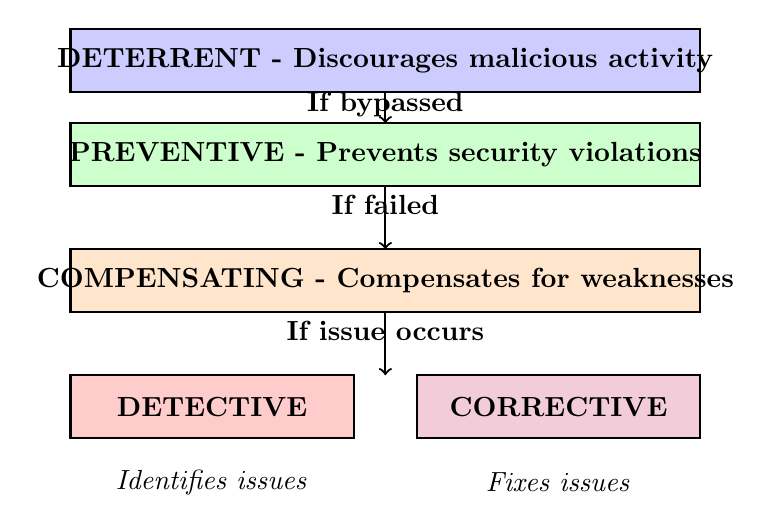
\begin{tikzpicture}[scale=0.8]
				% Deterrent
				\draw[thick, fill=blue!20] (0,0) rectangle (10,1) node[midway] {\textbf{DETERRENT - Discourages malicious activity}};
				
				% Arrow to preventive
				\draw[->, thick] (5,0) -- (5,-0.5);
				\node at (5,-0.2) {\textbf{If bypassed}};
				
				% Preventive
				\draw[thick, fill=green!20] (0,-1.5) rectangle (10,-0.5) node[midway] {\textbf{PREVENTIVE - Prevents security violations}};
				
				% Arrow to compensating
				\draw[->, thick] (5,-1.5) -- (5,-2.5);
				\node at (5,-1.8) {\textbf{If failed}};
				
				% Compensating
				\draw[thick, fill=orange!20] (0,-3.5) rectangle (10,-2.5) node[midway] {\textbf{COMPENSATING - Compensates for weaknesses}};
				
				% Arrow to detective/corrective
				\draw[->, thick] (5,-3.5) -- (5,-4.5);
				\node at (5,-3.8) {\textbf{If issue occurs}};
				
				% Detective and Corrective
				\draw[thick, fill=red!20] (0,-5.5) rectangle (4.5,-4.5) node[midway] {\textbf{DETECTIVE}};
				\draw[thick, fill=purple!20] (5.5,-5.5) rectangle (10,-4.5) node[midway] {\textbf{CORRECTIVE}};
				\node at (2.25,-6.2) {\textit{Identifies issues}};
				\node at (7.75,-6.2) {\textit{Fixes issues}};
			\end{tikzpicture}
		\end{center}
	\end{frame}
	
	\begin{frame}{4.1 Control Examples}
		\begin{block}{Detective vs Corrective Trap}
			\begin{itemize}
				\item \textbf{Common Mistake}: Confusing logging with restoring
				\item \textbf{Correct}: 
				\begin{itemize}
					\item \textbf{IDS detects} = Detective
					\item \textbf{Backup restore} = Corrective
				\end{itemize}
				\item \textbf{Why}: Detection happens \textit{during}; correction happens \textit{after}
			\end{itemize}
		\end{block}
		
		\begin{block}{Deterrent vs Preventive Trap}
			\begin{itemize}
				\item \textbf{Common Mistake}: Thinking cameras "prevent" intrusion
				\item \textbf{Correct}: 
				\begin{itemize}
					\item \textbf{Security cameras} = Deterrent (discourages)
					\item \textbf{Access control} = Preventive (stops)
				\end{itemize}
				\item \textbf{Why}: Deterrent works through \textit{psychology}; Preventive works through \textit{mechanics}
			\end{itemize}
		\end{block}
	\end{frame}
	
	% ----------------------------------------------------------------------
	\subsection{4.2 Control Implementation Techniques}
	\begin{frame}{4.2 Implementation Techniques}
		\begin{block}{Three Changeover Methods}
			\begin{tabular}{|p{2.5cm}|p{4cm}|p{4.5cm}|}
				\hline
				\textbf{Method} & \textbf{Description} & \textbf{Risk Level} \\
				\hline
				\textbf{Parallel} & Both systems run simultaneously & \textbf{Lowest} \\
				\hline
				\textbf{Phased} & Gradual replacement & \textbf{Medium} \\
				\hline
				\textbf{Abrupt} & Instant replacement & \textbf{Highest} \\
				\hline
			\end{tabular}
		\end{block}
		
		\begin{block}{Parallel Changeover}
			\begin{itemize}
				\item Both old and new systems run \textbf{simultaneously}
				\item \textbf{Safest} method
				\item Easy to \textbf{roll back}
				\item \textbf{No downtime}
				\item Allows \textbf{training} on new system
				\item \textbf{Drawback}: Expensive (maintaining both systems)
			\end{itemize}
		\end{block}
	\end{frame}
	
	\begin{frame}{4.2 Phased and Abrupt Changeover}
		\begin{block}{Phased Changeover}
			\begin{itemize}
				\item New systems implemented \textbf{gradually}
				\item Modules replaced \textbf{one at a time}
				\item More \textbf{cost-effective} than parallel
				\item \textbf{Reduced risk} of full system outage
				\item \textbf{Drawback}: Maintaining separate environments
			\end{itemize}
		\end{block}
		
		\begin{block}{Abrupt Changeover}
			\begin{itemize}
				\item Old systems \textbf{instantly} replaced
				\item \textbf{Fastest} method
				\item Most \textbf{cost-effective}
				\item \textbf{Drawback}: \textbf{Highest risk} - complete rollback may be required
				\item \textbf{Only} for non-critical systems
			\end{itemize}
		\end{block}
		
		\begin{alertblock}{The Critical Trap}
			\begin{itemize}
				\item \textbf{Business-critical systems} with no downtime tolerance = \textbf{PARALLEL}
				\item \textbf{Independent modules} with no dependencies = \textbf{PHASED}
				\item \textbf{Minor changes} with easy rollback = \textbf{ABRUPT}
			\end{itemize}
		\end{alertblock}
	\end{frame}
	
	% ============================================================
	% SECTION 5: RISK AND CONTROL MONITORING
	% ============================================================
	\section{5. Risk and Control Monitoring}
	
	% ----------------------------------------------------------------------
	\subsection{5.1 Key Indicators}
	\begin{frame}{5.1 KRI vs KPI vs KCI}
		\begin{block}{Three Key Metrics}
			\begin{tabular}{|p{2.5cm}|p{4cm}|p{4.5cm}|}
				\hline
				\textbf{Metric} & \textbf{Purpose} & \textbf{Example} \\
				\hline
				\textbf{KRI} & Predict future risk & \% of open vulnerabilities \\
				\hline
				\textbf{KPI} & Measure performance & System uptime \% \\
				\hline
				\textbf{KCI} & Measure control effectiveness & \% of access reviews completed \\
				\hline
			\end{tabular}
		\end{block}
		
		\begin{alertblock}{The Critical Trap}
			\begin{itemize}
				\item \textbf{KRIs} = \textit{Early Warning Signals} - Look \textbf{forward}
				\item \textbf{KPIs} = \textit{Performance Indicators} - Look \textbf{backward}
				\item \textbf{KCIs} = \textit{Control Effectiveness} - Measure if controls are \textbf{working}
			\end{itemize}
		\end{alertblock}
	\end{frame}
	
	\begin{frame}{5.1 SMART Metrics}
		\begin{block}{SMART Characteristics}
			\begin{tabular}{|p{2.5cm}|p{8.5cm}|}
				\hline
				\textbf{Letter} & \textbf{Meaning} \\
				\hline
				\textbf{S}pecific & Clearly understandable and concise \\
				\hline
				\textbf{M}easurable & Can be measured and quantified \\
				\hline
				\textbf{A}ttainable & Realistic and based on goals \\
				\hline
				\textbf{R}elevant & Relevant to a specific activity or goal \\
				\hline
				\textbf{T}imely & Timebound and not open-ended \\
				\hline
			\end{tabular}
		\end{block}
		
		\begin{exampleblock}{Key Insight}
			A key indicator should be \textbf{actionable}. \\
			If it can't drive action, it's not worth tracking.
		\end{exampleblock}
	\end{frame}
	
	\begin{frame}{5.1 KRI Maintenance}
		\begin{block}{Why Maintain KRIs?}
			\begin{itemize}
				\item Threats and vulnerabilities \textbf{change over time}
				\item Risk environment is \textbf{dynamic}
				\item KRIs must \textbf{evolve} with threats
				\item Ensure KRIs continue to \textbf{capture changes}
			\end{itemize}
		\end{block}
		
		\begin{alertblock}{The Critical Trap}
			\begin{itemize}
				\item \textbf{Not} for avoiding risk
				\item \textbf{Not} for fine-tuning complex metrics
				\item \textbf{Not} for timely reporting
				\item \textbf{Yes}: Because \textbf{threats and vulnerabilities change over time}
			\end{itemize}
		\end{alertblock}
	\end{frame}
	
	% ----------------------------------------------------------------------
	\subsection{5.2 Control Monitoring}
	\begin{frame}{5.2 Purpose of Control Monitoring}
		\begin{block}{Control Monitoring}
			\begin{itemize}
				\item Verify control is \textbf{effectively addressing} the risk
				\item NOT just checking if control is "working"
				\item Ensure controls remain \textbf{relevant}
				\item Identify \textbf{gaps} and \textbf{deficiencies}
			\end{itemize}
		\end{block}
		
		\begin{alertblock}{The Critical Trap}
			\textbf{Common Mistake}: Monitoring if the control is "working."
			
			\textbf{Correct}: Monitoring if the control is \textbf{effectively addressing the risk}.
			
			\textbf{Why}: A control can be "working" but not reducing risk!
		\end{alertblock}
	\end{frame}
	
	\begin{frame}{5.2 Control Assessment Techniques}
		\begin{block}{Assessment Methods}
			\begin{itemize}
				\item \textbf{Self-assessments} (MSIIs) - Internal risk assessments
				\item \textbf{Internal IS audit} - Independent evaluation
				\item \textbf{Vulnerability assessments} - Identify weaknesses
				\item \textbf{Penetration testing} - Simulate real attacks
				\item \textbf{Third-party assurance} - External audits
			\end{itemize}
		\end{block}
		
		\begin{block}{Penetration Testing Types}
			\begin{itemize}
				\item \textbf{White-box}: All information provided
				\item \textbf{Gray-box}: Some information provided
				\item \textbf{Black-box}: No information provided
			\end{itemize}
		\end{block}
	\end{frame}
	
	% ============================================================
	% SECTION 6: RISK REPORTING
	% ============================================================
	\section{6. Risk Reporting}
	
	% ----------------------------------------------------------------------
	\subsection{6.1 Reporting Formats}
	\begin{frame}{6.1 Risk Reporting Formats}
		\begin{block}{Four Reporting Formats}
			\begin{tabular}{|p{2.5cm}|p{4cm}|p{4.5cm}|}
				\hline
				\textbf{Format} & \textbf{Description} & \textbf{Best For} \\
				\hline
				\textbf{Executive Summary} & Concise, 1-2 pages & Quick updates \\
				\hline
				\textbf{Heat Map} & Graphical, color-coded & Visual risk levels \\
				\hline
				\textbf{Scorecard} & Aggregated grades & Performance tracking \\
				\hline
				\textbf{Dashboard} & Multiple metrics & Comprehensive view \\
				\hline
			\end{tabular}
		\end{block}
		
		\begin{block}{Dashboard Characteristics}
			\begin{itemize}
				\item Combines \textbf{qualitative} and \textbf{quantitative}
				\item Most \textbf{flexible} format
				\item Includes \textbf{multiple} indicators
				\item Enables \textbf{trend identification}
				\item Preferred method for \textbf{risk reporting}
			\end{itemize}
		\end{block}
	\end{frame}
	
	\begin{frame}{6.1 Effective Reporting Considerations}
		\begin{block}{Key Considerations}
			\begin{itemize}
				\item \textbf{Audience}: Who is the right audience?
				\item \textbf{Actionability}: Are metrics actionable?
				\item \textbf{Format}: Is the format appropriate?
				\item \textbf{Succinctness}: Is it concise and relevant?
				\item \textbf{Source}: Is the data source reliable?
				\item \textbf{Tailoring}: Is it relevant to stakeholders?
				\item \textbf{Timeframe}: Is the timeframe appropriate?
				\item \textbf{Inferences}: Can stakeholders draw insights?
				\item \textbf{Cadence}: Is the reporting frequency agreed?
			\end{itemize}
		\end{block}
	\end{frame}
	
	% ============================================================
	% SECTION 7: EXCEPTION MANAGEMENT
	% ============================================================
	\section{7. Exception Management}
	
	% ----------------------------------------------------------------------
	\subsection{7.1 Managing Exceptions}
	\begin{frame}{7.1 Exception Management}
		\begin{block}{What is an Exception?}
			\begin{itemize}
				\item \textbf{Deviation} from policy or standard
				\item Must be \textbf{formally documented}
				\item Must be \textbf{approved} by appropriate authority
				\item Brings \textbf{unknown risk} to the organization
				\item Must be \textbf{reviewed} periodically (at least annually)
			\end{itemize}
		\end{block}
		
		\begin{alertblock}{The Critical Trap}
			\textbf{Common Mistake}: Thinking exceptions are "bad."
			
			\textbf{Correct}: Exceptions are sometimes \textbf{necessary} for business reasons.
			
			\textbf{But}: They must be \textbf{managed} and \textbf{monitored}, not ignored!
		\end{alertblock}
	\end{frame}
	
	\begin{frame}{7.1 Change Management}
		\begin{block}{The Change Advisory Board (CAB)}
			\begin{itemize}
				\item Reviews and approves \textbf{changes}
				\item Includes \textbf{representatives} from multiple departments
				\item Ensures changes are \textbf{controlled}
				\item Balances \textbf{security} with \textbf{business needs}
			\end{itemize}
		\end{block}
		
		\begin{block}{CAB Verifications}
			\begin{itemize}
				\item Change won't \textbf{negatively affect} risk profile
				\item Change is \textbf{formally requested} and \textbf{justified}
				\item Change is \textbf{scheduled} at convenient time
				\item All \textbf{stakeholders} are informed
				\item Testing and \textbf{rollback plan} exist
				\item Change won't \textbf{compromise} security baselines
			\end{itemize}
		\end{block}
	\end{frame}
	
	% ============================================================
	% SECTION 8: COMMON EXAM TRAPS
	% ============================================================
	\section{8. Common Exam Traps}
	
	% ----------------------------------------------------------------------
	\subsection{8.1 Response and Monitoring Traps}
	\begin{frame}{8.1 Common Exam Traps - Risk Response}
		\begin{block}{Trap \#1: Mitigate vs Transfer}
			\begin{itemize}
				\item \textbf{Common Mistake}: Thinking outsourcing is always transfer
				\item \textbf{Correct}: 
				\begin{itemize}
					\item \textbf{Outsourcing} = Mitigation if risk remains
					\item \textbf{Transfer} = Contract shifts liability
				\end{itemize}
				\item \textbf{Example}: Hiring IT support = mitigation; Buying insurance = transfer
			\end{itemize}
		\end{block}
		
		\begin{block}{Trap \#2: Accept vs Avoid}
			\begin{itemize}
				\item \textbf{Common Mistake}: Confusing "doing nothing" with "eliminating"
				\item \textbf{Correct}: 
				\begin{itemize}
					\item \textbf{Avoidance} = Active elimination
					\item \textbf{Acceptance} = Passive retention
				\end{itemize}
				\item \textbf{Example}: Not doing e-commerce = avoid; Not fixing vulnerability = accept
			\end{itemize}
		\end{block}
	\end{frame}
	
	\begin{frame}{8.1 More Common Traps}
		\begin{block}{Trap \#3: Risk Owner vs Control Owner}
			\begin{itemize}
				\item \textbf{Common Mistake}: Thinking they are the same
				\item \textbf{Correct}: 
				\begin{itemize}
					\item \textbf{Risk Owner} = Accountable for risk treatment
					\item \textbf{Control Owner} = Responsible for control implementation
				\end{itemize}
			\end{itemize}
		\end{block}
		
		\begin{block}{Trap \#4: KRI vs KPI}
			\begin{itemize}
				\item \textbf{Common Mistake}: Using terms interchangeably
				\item \textbf{Correct}: 
				\begin{itemize}
					\item \textbf{KRIs} = Predict risk (forward-looking)
					\item \textbf{KPIs} = Measure performance (backward-looking)
				\end{itemize}
			\end{itemize}
		\end{block}
	\end{frame}
	
	% ============================================================
	% SECTION 9: QUICK REFERENCE
	% ============================================================
	\section{9. Quick Reference}
	
	% ----------------------------------------------------------------------
	\subsection{9.1 Response and Reporting Reference}
	\begin{frame}{9.1 Quick Reference - Risk Response}
		\begin{block}{Response Strategies}
			\begin{tabular}{|p{2.5cm}|p{4cm}|p{4.5cm}|}
				\hline
				\textbf{Strategy} & \textbf{Action} & \textbf{Example} \\
				\hline
				\textbf{Mitigate} & Reduce probability/impact & Implement controls \\
				\hline
				\textbf{Accept} & Acknowledge and monitor & Formal sign-off \\
				\hline
				\textbf{Transfer} & Shift to third party & Insurance, outsourcing \\
				\hline
				\textbf{Avoid} & Eliminate entirely & Terminate project \\
				\hline
			\end{tabular}
		\end{block}
		
		\begin{block}{Control Types}
			\begin{tabular}{|p{2.5cm}|p{4cm}|p{4.5cm}|}
				\hline
				\textbf{Type} & \textbf{Timing} & \textbf{Example} \\
				\hline
				Preventive & Before event & Firewall, Encryption \\
				\hline
				Detective & During event & IDS, Log monitoring \\
				\hline
				Corrective & After event & Backup restore \\
				\hline
				Deterrent & Before event & Security cameras \\
				\hline
				Compensating & Ongoing & Additional oversight \\
				\hline
			\end{tabular}
		\end{block}
	\end{frame}
	
	\begin{frame}{9.1 Quick Reference - Reporting}
		\begin{block}{Key Indicators}
			\begin{tabular}{|p{2.5cm}|p{4cm}|p{4.5cm}|}
				\hline
				\textbf{Type} & \textbf{Purpose} & \textbf{Direction} \\
				\hline
				KRI & Predict risk & Forward-looking \\
				\hline
				KPI & Measure performance & Backward-looking \\
				\hline
				KCI & Measure control effectiveness & Current/Historical \\
				\hline
			\end{tabular}
		\end{block}
		
		\begin{block}{Reporting Formats}
			\begin{itemize}
				\item \textbf{Executive Summary}: Concise, text-based
				\item \textbf{Heat Map}: Visual, qualitative only
				\item \textbf{Scorecard}: Aggregated, qualitative
				\item \textbf{Dashboard}: Comprehensive, \textbf{both qualitative and quantitative}
			\end{itemize}
		\end{block}
	\end{frame}
	
	\begin{frame}{9.1 Exam Success Tips}
		\begin{block}{Response Section Strategy}
			\begin{itemize}
				\item \textbf{Remember the 4 Rs}: Mitigate, Accept, Transfer, Avoid
				\item \textbf{Cost-Benefit}: If control cost > expected loss, Accept
				\item \textbf{Exceptions}: Must be documented and reviewed annually
				\item \textbf{Change Management}: CAB must include all relevant stakeholders
				\item \textbf{KRI Maintenance}: Because threats change over time
				\item \textbf{Control Monitoring}: Verify risk mitigation, not just operation
			\end{itemize}
		\end{block}
		
		\begin{exampleblock}{The ISACA Mindset for Response}
			\centering
			\Large{\textbf{Business Enablement First}}
			
			\normalsize{The goal is NOT to eliminate risk but to \textbf{optimize} it.}
		\end{exampleblock}
	\end{frame}
	
	\begin{frame}{Final Advice - Section 3}
		\begin{block}{Risk Response and Reporting}
			\centering
			\vspace{0.3cm}
			\textbf{Remember:}
			\begin{itemize}
				\item \textbf{Mitigate} = Reduce risk (not eliminate)
				\item \textbf{Accept} = Formal, documented, management approval
				\item \textbf{Transfer} = Insurance or outsourcing (accountability remains)
				\item \textbf{Avoid} = Eliminate entirely (ONLY strategy that does so)
				\item \textbf{KRIs} = Predict risk; \textbf{KPIs} = Measure performance
				\item \textbf{Control Monitoring} = Verify risk mitigation, not operation
				\item \textbf{Exceptions} = Must be formally approved and reviewed
			\end{itemize}
			\vspace{0.5cm}
			\textbf{Next: Section 4 - Information Technology and Security}
		\end{block}
	\end{frame}
	
	% ============================================================
	% END OF PRESENTATION
	% ============================================================
	
\end{document}